\usepackage{style}
\usepackage{url}

\title[SOR in Snow Simulation]{SOR method in Snow Simulation on GPUs}
\author{Hallgeir Lien}
\begin{document}

\maketitle

\AtBeginSection{
    \begin{frame}
    \tableofcontents[currentsection]
    \end{frame}
}

\begin{frame}
\frametitle{Outline}
\tableofcontents
\end{frame}

% Project description
\section{My project}

\begin{frame}
\frametitle{My project}
My project has several parts:
\begin{itemize}
\item Given a terrain, automatically generate a road that minimizes a cost function based on slope and curvature.
\item Extending the wind simulator at the HPC lab to support meshes, e.g. roads through the terrain.
\item Import real world maps into the simulator.
\item If time, use snow height data from simulator as a part of the cost function when generating roads.
\item Also interesting: How is snow built up after it's removed from the road?
\end{itemize}
\end{frame}

\begin{frame}
\frametitle{Road generation}
I use the method described in Galin et. al.: Procedural road generation.
\begin{itemize}
\item Uses an A* search through the terrain, from a start to an endpoint.
\item Terrain is discretized into a grid.
\item Cost to go from gridpoint $\mathbf{p}_a$ to $\mathbf{p}_b$ is determined by a cost function.
\item Cost based on slope, curvature of the road, and length of the road.
\item Possibly soon: Also dependent on potential snow height.
\end{itemize}
\end{frame}

\begin{frame}
\frametitle{Real world maps}
Elevation maps from Kartverket is to be imported.
\begin{itemize}
\item Maps often come in the USGS DEM (US Geological Survey Digital Elevation Map) format.
\item An inconvenient format: Not a rectangular map, often skewed, space demanding (in ASCII)
\item These must be converted to a more reasonable format, e.g. a 16 bit RAW format.
\end{itemize}
\end{frame}

\begin{frame}
\frametitle{Real world maps}
\begin{figure}[ht]
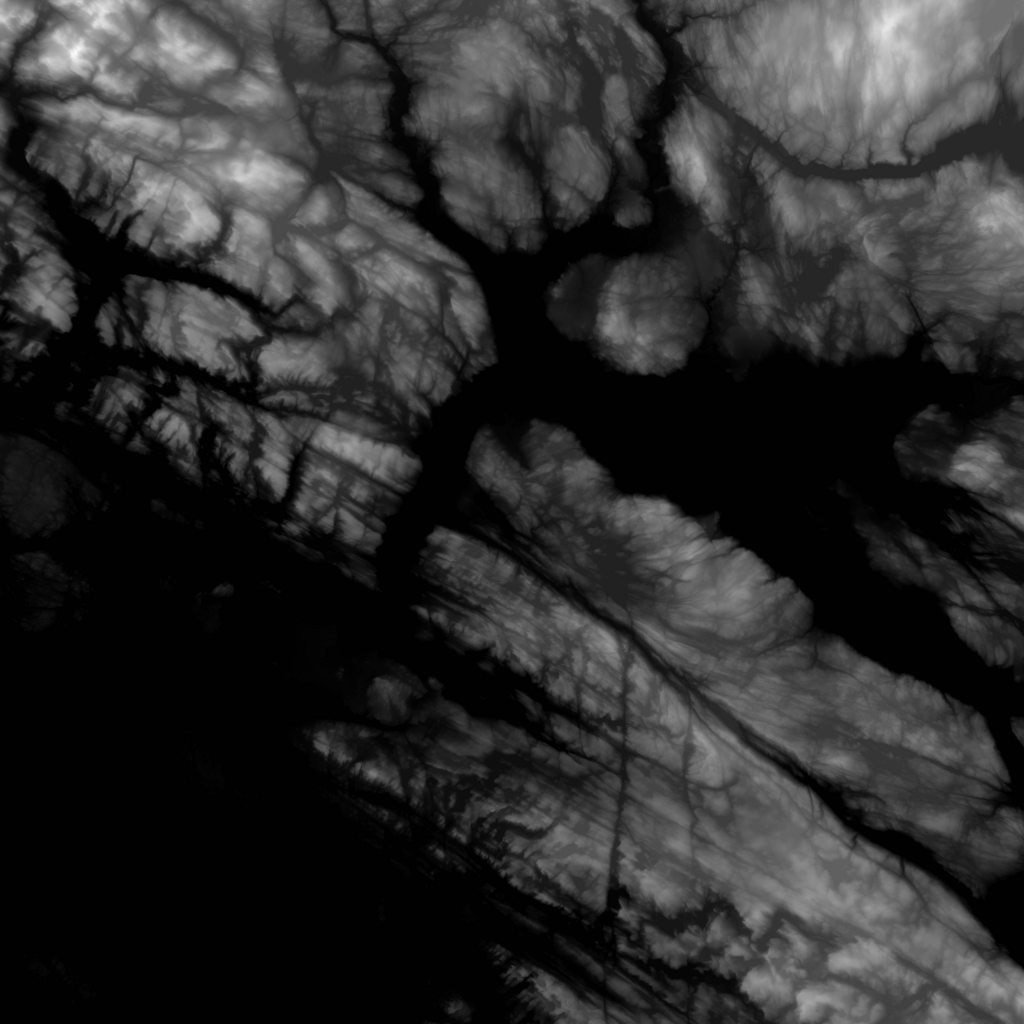
\includegraphics[width=0.75\textwidth]{gfx/converted_map}
\caption{Imported map}
\label{fig:trondheim}
\end{figure}
\end{frame}

\begin{frame}
\frametitle{Mesh support}
Currently, the only sort of models in the snow simulator is the terrain (Derived from a height map).
\begin{itemize}
\item At first, loading meshes into the snow simulator will be used to model roads.
\item Perhaps also famous landmarks for the real world terrains used (Space Needle in Seattle, Tyholt tower in Trondheim)
\end{itemize}
\end{frame}

\begin{frame}
\frametitle{Links}
\begin{description}
\item[Galin et. al.: Procedural road generation] \url{http://liris.cnrs.fr/~egalin/Pdf/2010-roads.pdf}
\item[Edissen: Utilizing GPUs for Real-Time Visualization of Snow] \url{http://www.idi.ntnu.no/\~elster/master-studs/robine/robin-eidissen-master-ntnu.pdf}
\item[Cvetanovic et. al.] \url{https://bioinformatics.cs.vt.edu/~guos/parallel/00205103.pdf}
%\item[A controlled clothoid spline] \url{http://imara.inria.fr/_media/users/franciscogarcia/a_controlled_clothoid_spline.pdf}
\end{description}
\end{frame}


\section{Solving linear equations}
\begin{frame}
\frametitle{Solving linear equations}
Solving linear equations of the form $A\bf{x} = \bf{b}$ is important in a lot of different simulations.

\begin{itemize}
\item In the snow simulator, simulating the wind field involves solving a linear system at each timestep.
\item Number of variables: Depends on the resolution of the wind field. In order of hundreds of thousands.
\item Solving exactly (with Gauss-Jordan) takes $O(n^3)$ time, $n$ is the number of variables.
\item Gauss elimination is WAY too slow for any practical applications for such large systems.
\end{itemize}

\end{frame}

\begin{frame}
\frametitle{An iterative method: Jacobi}
We don't need to solve $A\bf{x} = \bf{b}$ exactly; it can be done iteratively, until the solution is good enough.
\begin{itemize}
\item One method is the Jacobi method.
\item Slow convergence ($O(n^2)$ iterations; each iteration computes
$$
x_i^{(k+1)} = \frac{1}{a_{ii}}\left(b_i-\sum_{j\neq i} a_{i,j}x_j^{(k)}\right)
$$
\item REALLY easy to parallelize on a GPU: Just let each thread compute one element of $x_i^{k+1}$.
\end{itemize}

There are many other algorithms... (Multigrid, FFT, CG, SOR, Gauss-Seidel, ...).
\end{frame}

\begin{frame}
\frametitle{Gauss-Seidel and Successive Over-Relaxation (SOR)}
Observation: Already computed elements can be used immediately, before the next iteration. 
\begin{itemize}
\item One method is called Successive Over-Relaxation. For each unknown, compute:
$$
x_i^{(k+1)} = (1-\omega)x_i^{(k)} + \frac{\omega}{a_{ii}}\left(b_i-\sum_{j > i} a_{i,j}x_j^{(k)}-\sum_{j < i} a_{i,j}x_j^{(k+1)}\right)
$$
\item Gauss-Seidel is SOR with $\omega = 1$.
\item Parallelization is less straight forward, but still easy for many applications.
\end{itemize}

\end{frame}

\section{Linear equations in differential equations}

\begin{frame}
\frametitle{Discretizing differential equations}
Differential equations must be expressed in discrete quantities before being solved numerically (Computers suck at working with infinidesimal sizes...).

Differentials are approximated with finite difference methods. E.g. $\frac{dy}{dx}\approx \frac{y(x+h)-y(x-h)}{2h}$. Higher order derivatives require more points. E.g. $\frac{d^2y}{dx^2}\approx \frac{f(x+h)-2f(x)+f(x-h)}{h^2}$.

Example: The differential equation $\frac{dy}{dx} = y$ is approximated by $\frac{y(x+h)-y(x-h)}{2h} = y(x)$

\end{frame}

\begin{frame}
\frametitle{Discretizing partial differential equations}
Partial differential equations (differential equations with more than one variable) is discretized the same way as before, but in several dimensions.

Example: Poisson's equation in 2D: $\frac{\delta^2 u}{\delta x^2} + \frac{\delta^2 u}{\delta y^2} = f(x,y,t)$
Discretized into:
$$\Delta \varphi =
\frac{u(x+h,y,t)-2u(x,y,t)+u(x-h,y,t)}{h^2} + $$
$$
\frac{u(x,y+h,t)-2u(x,y,t)+u(x,y-h,t)}{h^2} = f(x,y,t)
$$

\end{frame}

\begin{frame}
\frametitle{SOR applied to differential equations}
Simple way of solving this: Use the Crank-Nicholson method. Notation: $U(i\pm 1,j\pm 1,t\pm 1)=u(x\pm h,y \pm h,t \pm h)$
Setting it up and rearranging gives
$$
(1+\frac{2k}{h^2})U(i,j,t+1)-\frac{k}{2h^2}(U(i-1,j,t+1)+U(i+1,j,t+1) + $$
$$(U(i,j-1,m+1) + U(i,j+1,m+1)) = b(i,j,t)
$$

where $b(i,j,t)$ is a combination of all the known values.

This becomes a linear system.

\end{frame}

\begin{frame}
\frametitle{SOR applied to differential equations}
With a grid size of $3\times 3$, the system 
$Ax=b$ becomes
$$
\left[
\begin{array}{ccccccccc}
4 & 1 & 0 & 1 & 0 & 0 & 0 & 0 & 0\\
1 & 4 & 1 & 0 & 1 & 0 & 0 & 0 & 0\\
0 & 1 & 4 & 0 & 0 & 1 & 0 & 0 & 0\\
1 & 0 & 0 & 4 & 1 & 0 & 1 & 0 & 0\\
0 & 1 & 0 & 1 & 4 & 1 & 0 & 1 & 0\\
0 & 0 & 1 & 0 & 1 & 4 & 0 & 0 & 1\\
0 & 0 & 0 & 1 & 0 & 0 & 4 & 1 & 0\\
0 & 0 & 0 & 0 & 1 & 0 & 1 & 4 & 1\\
0 & 0 & 0 & 0 & 0 & 1 & 0 & 1 & 4
\end{array}
\right]
\left[
\begin{array}{c}
U(1,1,t+1) \\
U(2,1,t+1) \\
U(3,1,t+1) \\
U(1,2,t+1) \\
U(2,2,t+1) \\
U(3,2,t+1) \\
U(1,3,t+1) \\
U(2,3,t+1) \\
U(3,3,t+1) 
\end{array}
\right]
=
\left[
\begin{array}{c}
b(1,1,t) \\
b(2,1,t) \\
b(3,1,t) \\
b(1,2,t) \\
b(2,2,t) \\
b(3,2,t) \\
b(1,3,t) \\
b(2,3,t) \\
b(3,3,t) 
\end{array}
\right]
$$
\end{frame}

\begin{frame}
\frametitle{SOR applied to differential equations}
From the expression for the SOR, using the matrix we saw:
$$
\begin{array}{ll}
U(i,j,t+1) = & (1-\omega)U(i,j,t) + \\
             & \frac{\omega}{4} (b(i,j,t) -  U(i-1,j,t) - \\
             & U(i,j+1,t) - U(i+1,j,t+1) - \\
             & U(i,j-1,t+1))
\end{array}
$$

More direct interpretation: Take four neighbors, take the average, and use that as the approximation for $U(u,j,t+1)$.

$\omega$ controls the convergence: 
\begin{itemize}
\item $\omega \in (1, 2]$ is overrelaxation (may give faster convergence)
\item $\omega = 1$ gives Jacobi
\item $\omega \in (0,1)$ gives underrelaxation (may make unstable systems converge)
\end{itemize}
\end{frame}

\begin{frame}
\frametitle{Parallelization of SOR}
Each unknown variable cannot be updated independently in SOR.
\begin{itemize}
\item Unfortunate for GPU implementations of SOR
\item However, there's a remedy: Red-black ordering (Example)
\end{itemize}
\end{frame}

\section{Snow simulation}
\begin{frame}
\frametitle{Overview}
The snow simulator has multiple parts:
\begin{enumerate}
\item Simulation of the wind field in a discrete 3D grid.
\item Simulation of the snow particles (updating their position based on wind, etc.)
\item Rendering.
\end{enumerate}
\end{frame}

\begin{frame}
\frametitle{Wind Simulation}
Wind is simulated as a fluid. Modelled by the Navier-Stokes equations:
$$
\begin{array}{rl}
\frac{\delta {\bf v}}{\delta t} = & -({\bf v}\cdot \nabla){\bf v}-\frac{1}{\rho}\nabla p + v\Delta {\bf v} + {\bf f}\\
\nabla\cdot {\bf v} = & 0
\end{array}
$$

\begin{description}
\item[Advection] $-({\bf v}\cdot \nabla){\bf v}$: Motion with the fluid (which moves at velocity ${\bf v}$), i.e. the fluid moves along its own flow.
\item[Pressure] $-\frac{1}{\rho}\nabla p$: The velocity field moves along the gradient of the pressure field.
\item[Diffusion] $v\Delta {\bf v}$.
\item[External forces] ${\bf f}$, is for example gravity.
\end{description}
\end{frame}

\begin{frame}
\frametitle{Wind Simulation}
Setting viscosity to 0, and density to 1, we get the Euler equations:
$$
\frac{\delta {\bf v}}{\delta t} = -({\bf v}\cdot \nabla){\bf v}-\nabla p 
$$

There are then 3 steps:
\begin{enumerate}
\item Advection: ${\bf F}^{(n)} = {\bf v}^{(n)} - \delta t({\bf v} \cdot \nabla){\bf v}$.
\item Solve Poisson's equation: $\Delta p^{(n+1)} = \frac{1}{\delta t}\nabla {\bf F}^{(n)}$
\item Compute pressure forces. Store result back in ${\bf v}$.
\end{enumerate}
\end{frame}

\begin{frame}
\frametitle{Snow particle simulation}
The snow particles are simulated in each step by, for each particle:
\begin{enumerate}
\item Looking up the wind velocity from a 3D texture
\item Computing drag, accelleration and finally the updated velocity
\item Computing rotation velocity.
\item Updating the position by incrementing the position by the velocity.
\item Check if the particle has collided. If yes, increase snow height at that point.
\end{enumerate}
\end{frame}


\end{document}
